Verificada a necessidade de efetuar a calibração, ou seja, fazer corresponder o valor digital obtido através do conversor analógico-digital ao valor de entrada do mesmo, utilizou-se o gerador de funções disponível no laboratório. Com este simulou-se uma fonte DC ao gerar um sinal com uma frequência e amplitude pico a pico praticamente nulas ($f\approx0$ e $V_{pp}\approx0$). Simulada esta fonte, alterou-se o valor do \textit{offset} na gama de valores $\{-5,-4,-3,-2,-1,0,1,2,3,4,5\}$ como é visível pelos pontos e escala das ordenadas da \autoref{fig:Reta de ajuste experimental}. 

\begin{figure}[H]
    \centering
    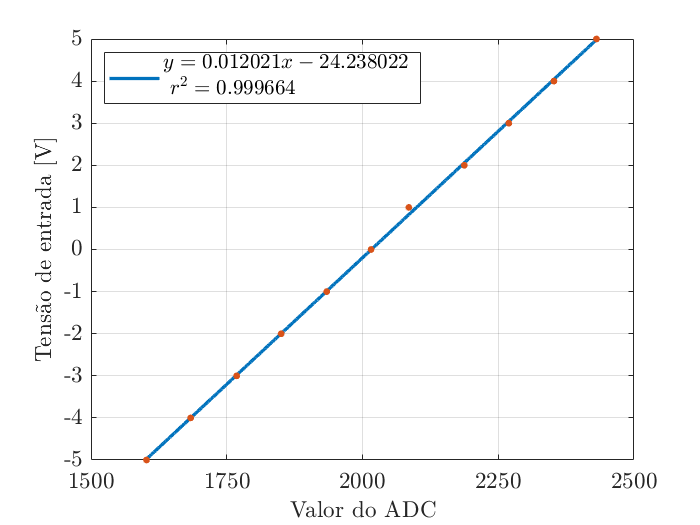
\includegraphics[width=0.47\textwidth]{Imagens/Testes no laboratório/Ajuste experimental/Calibração experimental.png}
    \captionsetup{justification=centering}
    \caption{Reta de ajuste experimental}
    \label{fig:Reta de ajuste experimental}
\end{figure}

À medida que se alteravam os valores usufruiu-se do \textit{script} \texttt{main\_exemplo\_2.py} para calcular a média de $100$ amostras cujos valores representam o eixo das abcissas da \autoref{fig:Reta de ajuste experimental}. Note-se que o gráfico acima é o inverso do apresentado no enunciado, pelo que no código da função \texttt{read\_and\_calculate()}, e já tendo a equação de ajuste, aparecem as linhas \texttt{73}, \texttt{74} e \texttt{75} comentadas e a \texttt{76} descomentada. Para confirmação do bom ajuste usou-se o \textit{script} \texttt{main\_exemplo\_1.py} com o qual se verificou que para uma tensão DC de $5$V o valor médio era $5.06$V ($\text{Erro}=1.2\%<5\%$ - indicação de bom ajuste).